% Options for packages loaded elsewhere
\PassOptionsToPackage{unicode}{hyperref}
\PassOptionsToPackage{hyphens}{url}
%
\documentclass[
  ignorenonframetext,
]{beamer}
\usepackage{pgfpages}
\setbeamertemplate{caption}[numbered]
\setbeamertemplate{caption label separator}{: }
\setbeamercolor{caption name}{fg=normal text.fg}
\beamertemplatenavigationsymbolsempty
% Prevent slide breaks in the middle of a paragraph
\widowpenalties 1 10000
\raggedbottom
\setbeamertemplate{part page}{
  \centering
  \begin{beamercolorbox}[sep=16pt,center]{part title}
    \usebeamerfont{part title}\insertpart\par
  \end{beamercolorbox}
}
\setbeamertemplate{section page}{
  \centering
  \begin{beamercolorbox}[sep=12pt,center]{part title}
    \usebeamerfont{section title}\insertsection\par
  \end{beamercolorbox}
}
\setbeamertemplate{subsection page}{
  \centering
  \begin{beamercolorbox}[sep=8pt,center]{part title}
    \usebeamerfont{subsection title}\insertsubsection\par
  \end{beamercolorbox}
}
\AtBeginPart{
  \frame{\partpage}
}
\AtBeginSection{
  \ifbibliography
  \else
    \frame{\sectionpage}
  \fi
}
\AtBeginSubsection{
  \frame{\subsectionpage}
}
\usepackage{lmodern}
\usepackage{amssymb,amsmath}
\usepackage{ifxetex,ifluatex}
\ifnum 0\ifxetex 1\fi\ifluatex 1\fi=0 % if pdftex
  \usepackage[T1]{fontenc}
  \usepackage[utf8]{inputenc}
  \usepackage{textcomp} % provide euro and other symbols
\else % if luatex or xetex
  \usepackage{unicode-math}
  \defaultfontfeatures{Scale=MatchLowercase}
  \defaultfontfeatures[\rmfamily]{Ligatures=TeX,Scale=1}
\fi
% Use upquote if available, for straight quotes in verbatim environments
\IfFileExists{upquote.sty}{\usepackage{upquote}}{}
\IfFileExists{microtype.sty}{% use microtype if available
  \usepackage[]{microtype}
  \UseMicrotypeSet[protrusion]{basicmath} % disable protrusion for tt fonts
}{}
\makeatletter
\@ifundefined{KOMAClassName}{% if non-KOMA class
  \IfFileExists{parskip.sty}{%
    \usepackage{parskip}
  }{% else
    \setlength{\parindent}{0pt}
    \setlength{\parskip}{6pt plus 2pt minus 1pt}}
}{% if KOMA class
  \KOMAoptions{parskip=half}}
\makeatother
\usepackage{xcolor}
\IfFileExists{xurl.sty}{\usepackage{xurl}}{} % add URL line breaks if available
\IfFileExists{bookmark.sty}{\usepackage{bookmark}}{\usepackage{hyperref}}
\hypersetup{
  pdftitle={ Smart Data Analytics: Prediction of Bitcoin and Ethereum Returns using Subreddits},
  pdfauthor={Luca Riboni, Daniil Bulat},
  hidelinks,
  pdfcreator={LaTeX via pandoc}}
\urlstyle{same} % disable monospaced font for URLs
\newif\ifbibliography
\usepackage{graphicx,grffile}
\makeatletter
\def\maxwidth{\ifdim\Gin@nat@width>\linewidth\linewidth\else\Gin@nat@width\fi}
\def\maxheight{\ifdim\Gin@nat@height>\textheight\textheight\else\Gin@nat@height\fi}
\makeatother
% Scale images if necessary, so that they will not overflow the page
% margins by default, and it is still possible to overwrite the defaults
% using explicit options in \includegraphics[width, height, ...]{}
\setkeys{Gin}{width=\maxwidth,height=\maxheight,keepaspectratio}
% Set default figure placement to htbp
\makeatletter
\def\fps@figure{htbp}
\makeatother
\setlength{\emergencystretch}{3em} % prevent overfull lines
\providecommand{\tightlist}{%
  \setlength{\itemsep}{0pt}\setlength{\parskip}{0pt}}
\setcounter{secnumdepth}{-\maxdimen} % remove section numbering

\title{
\includegraphics[width=1in,height=\textheight]{unisg_logo.jpg}\\
Smart Data Analytics: Prediction of Bitcoin and Ethereum Returns using
Subreddits}
\author{Luca Riboni, Daniil Bulat}
\date{December 2020}

\begin{document}
\frame{\titlepage}

\begin{frame}{Introduction}
\protect\hypertarget{introduction}{}

In our project we want to test the predictive power of Reddit
submissions on the returns of cryptocurrencies. First, submission data
from the Reddit websites Bitcoin and Ethereum Subreddits was collected
from 2015 until December 2020. Then a sentiment analysis on the
submission titles and the submission texts was run using the XXYY
dictionary. As there are numerous submissions per day, the daily /
weekly / monthly sentiment score is the mean sentiment of all
submissions per day / week / month, weighted by the number of
``upvotes'' each submission received. In a final step OLS regression
with three independent variables is used to test the predictive power of
Reddit submissions on daily Bitcoin and Ethereum returns. The returns
being the dependent variable and daily, weekly and monthly sentiment
scores being the independent variables. Todays returns are regressed on
yesterdays, previous weeks and previous months sentiment score.

\end{frame}

\begin{frame}{Reddit}
\protect\hypertarget{reddit}{}

Reddit is a social news aggregation and discussion website. It is a
major discussion forum for crypto related content. Users have only
limited restrictions to contributing content on the website allowing a
very free sharing of information. Due to the lack of cryptocurrencie
coverage by traditional media, many investors seek advise and
information regarding cryptos on Reddit and similar websites. Therefore,
Reddit submissions were chosen as predictors for this project.

\end{frame}

\begin{frame}{Sentiment Analysis}
\protect\hypertarget{sentiment-analysis}{}

\end{frame}

\begin{frame}{Word Clouds}
\protect\hypertarget{word-clouds}{}

\end{frame}

\begin{frame}{OLS Regression}
\protect\hypertarget{ols-regression}{}

\begin{figure}
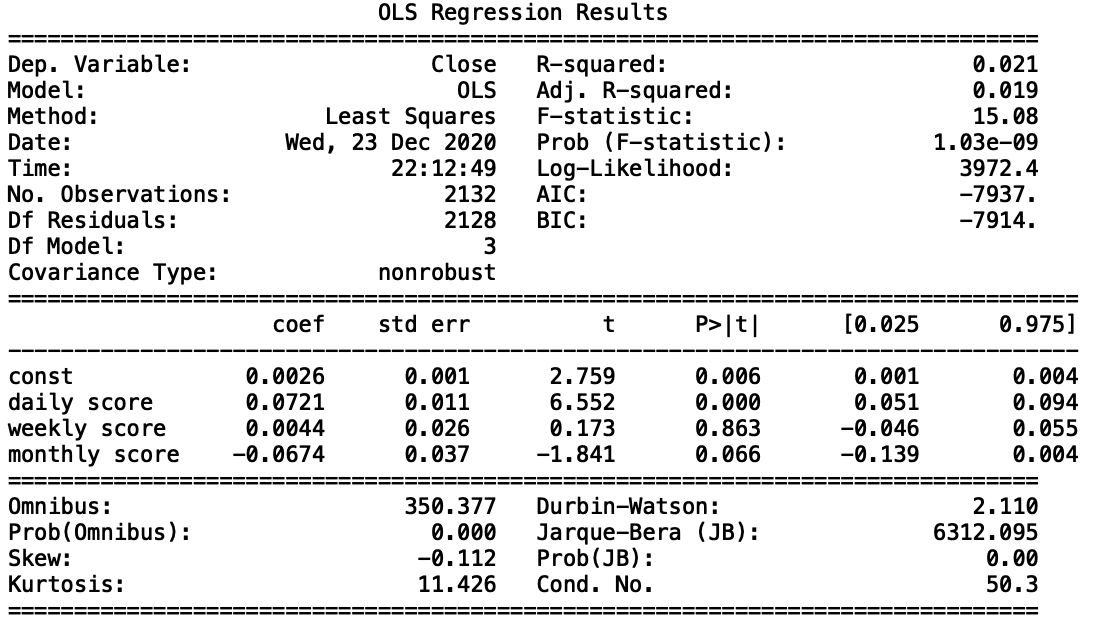
\includegraphics[width=1\linewidth]{btc_ols} \caption{A caption}\label{fig:pressure-1}
\end{figure}
\begin{figure}
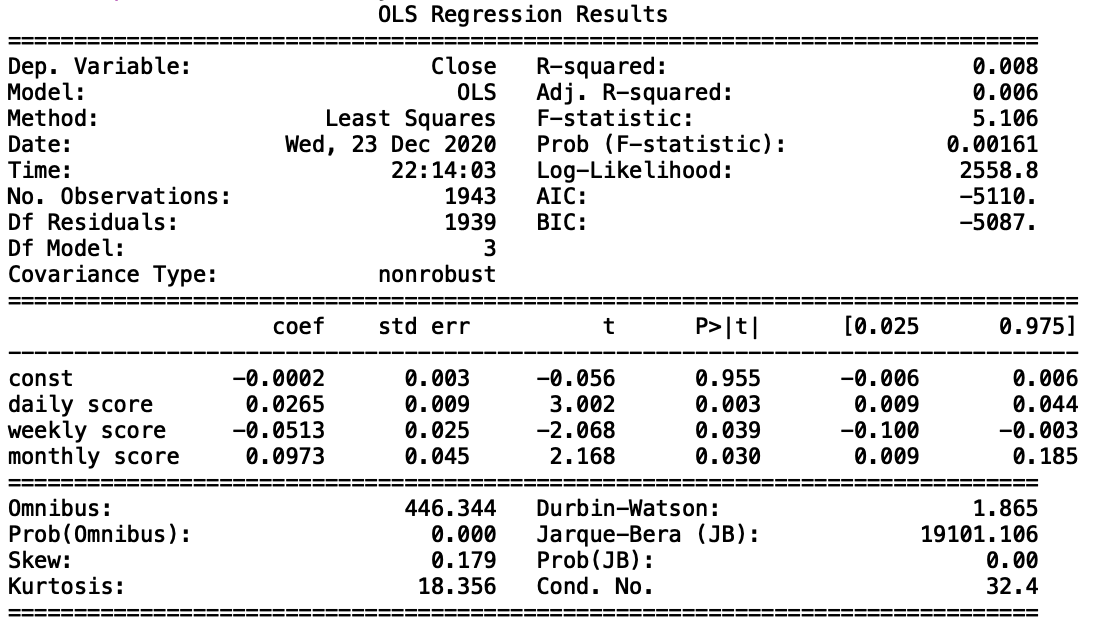
\includegraphics[width=1\linewidth]{eth_ols} \caption{A caption}\label{fig:pressure-2}
\end{figure}

\end{frame}

\begin{frame}{Results}
\protect\hypertarget{results}{}

\end{frame}

\end{document}
